\RequirePackage{luatex85}
\documentclass[tikz, border=10pt]{standalone}
\usetikzlibrary{shapes.geometric, arrows}
\usetikzlibrary{positioning}

\tikzstyle{tagger} = [rectangle, rounded corners, minimum width=3cm, minimum height=1.2cm, text centered, text width=3.5cm, draw=black, fill=white]

\tikzstyle{high_level_tagger} = [regular polygon,regular polygon sides=4, rounded corners, minimum width=1cm, text centered, text width=3.5cm, draw=black, fill=white]

\tikzstyle{arrow} = [thick,->,>=stealth]

\begin{document}

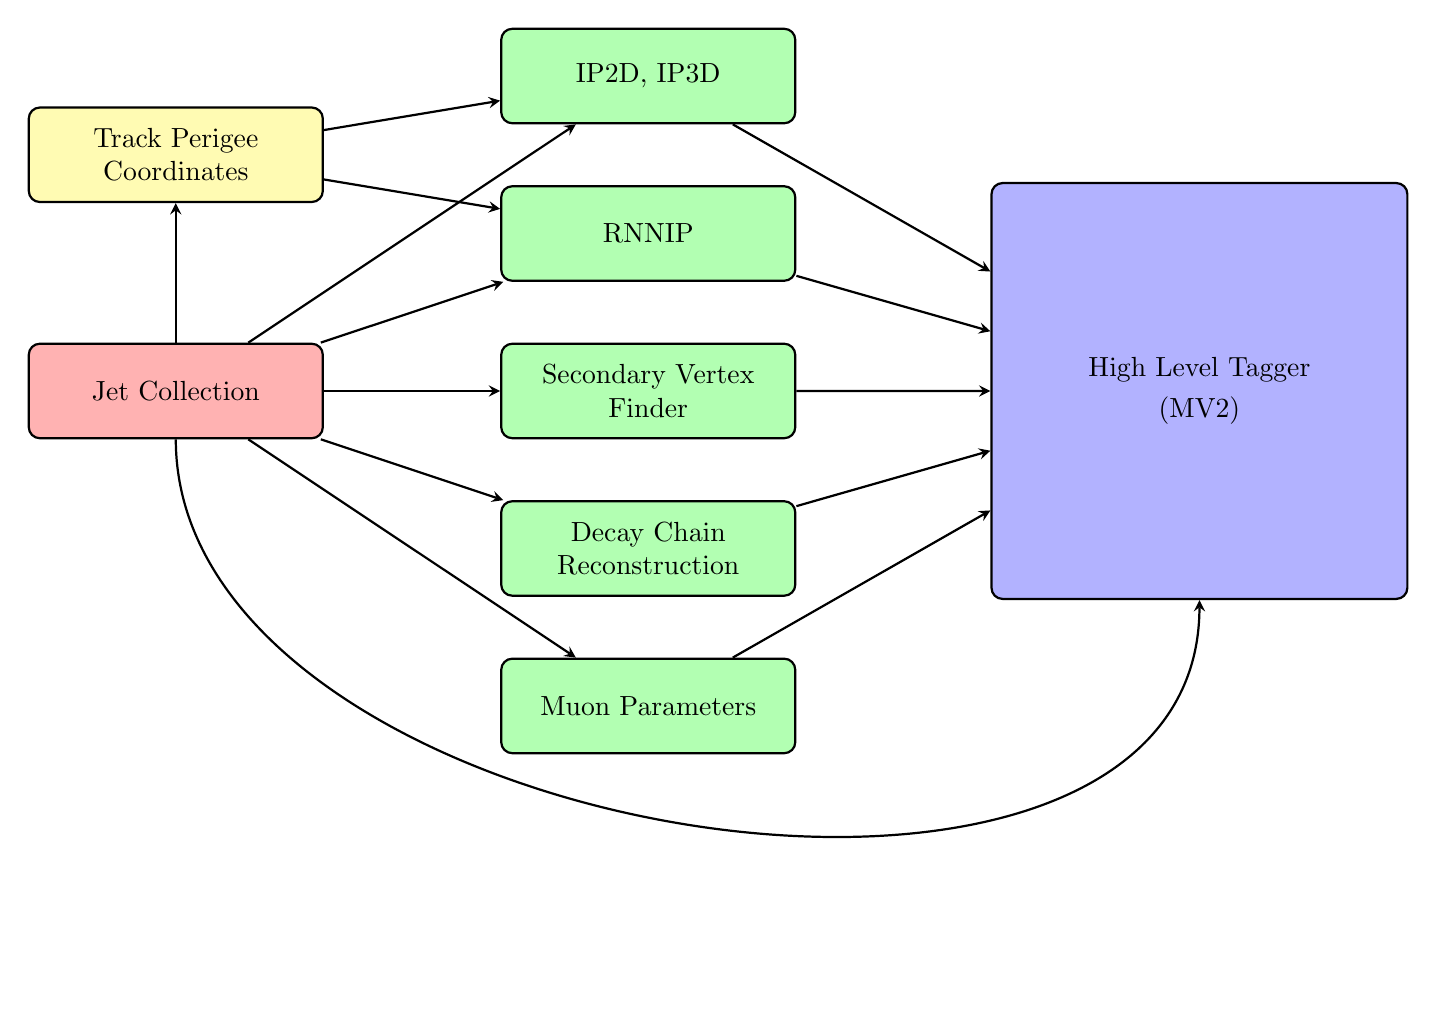
\begin{tikzpicture}[thick, node distance=2cm]
 \node (jet_collection) [tagger, fill=red!30] {Jet Collection};
 \node (track_coordinates) [tagger, above of=jet_collection, node distance=3cm, fill=yellow!30] {Track Perigee\\Coordinates};
 \node (SV1) [tagger, right of=jet_collection, node distance=6cm, fill=green!30] {Secondary Vertex\\Finder};
 \node (IP3D) [tagger, above of=SV1, node distance=4cm, fill=green!30] {IP2D, IP3D};
 \node (RNNIP) [tagger, above of=SV1, node distance=2cm, fill=green!30] {RNNIP};
 \node (JetFitter) [tagger, below of=SV1, node distance=2cm, fill=green!30] {Decay Chain\\Reconstruction};
 \node (SMT) [tagger, below of=SV1, node distance=4cm, fill=green!30] {Muon Parameters};

 \node (MV2) [high_level_tagger, right of=SV1, node distance=7cm, fill=blue!30] {High Level Tagger\\\vspace{3pt}(MV2)};

 \draw [arrow] (jet_collection) -- (IP3D);
 \draw [arrow] (jet_collection) -- (RNNIP);

 \draw [arrow] (jet_collection) -- (track_coordinates);
 \draw [arrow] (track_coordinates) -- (IP3D);
 \draw [arrow] (track_coordinates) -- (RNNIP);

 \draw [arrow] (jet_collection) -- (SV1);
 \draw [arrow] (jet_collection) -- (JetFitter);
 \draw [arrow] (jet_collection) -- (SMT);

 \draw [arrow] (jet_collection.south) to [out=-90,in=-90] (MV2.south);
 \draw [arrow] (IP3D) -- (MV2);
 \draw [arrow] (RNNIP) -- (MV2);
 \draw [arrow] (SV1) -- (MV2);
 \draw [arrow] (JetFitter) -- (MV2);
 \draw [arrow] (SMT) -- (MV2);

\end{tikzpicture}
\end{document}
